\documentclass[11pt,a4paper]{article}
\usepackage[utf8]{inputenc}
\usepackage[english]{babel}
\usepackage{graphicx}
\usepackage{hyperref}
\usepackage{geometry}
\usepackage{float} 
\geometry{margin=1in}

% 告诉 LaTeX 图片在 'png' 这个文件夹里找
\graphicspath{ {./png/} }

\title{\textbf{OpTime: Front-End Development Report}}
\author{Haonan Wu (126815),
Ruyue Zhao (127561) \vspace{0.3cm}\\
Project: Optimising Timetables (WiSe 2025) \\
Advisor: Andreas Jakoby}
\date{}

\begin{document}

\maketitle

\section{UI/UX Design \& User Experience}

\subsection{Information Hierarchy and Navigation}
The OpTime application follows a \textbf{Dashboard-Centric} layout designed for maximum administrative efficiency. The visual architecture is structured to ensure that critical navigation and data operations are always within one click of the user's focus (see Figure \ref{fig:dashboard}).
\begin{itemize}
    \item \textbf{Global Navigation}: The left-hand sidebar serves as the primary router, allowing instant switching between \textbf{Lecturers}, \textbf{Courses}, and \textbf{Rooms}. This persistent placement ensures that the user never loses their sense of "location" within the data hierarchy.
    \item \textbf{Version Control (Saved Schedules)}: A standout feature is the \textbf{Saved Schedules} repository in the sidebar. It tracks historical schedule generations with precise timestamps (e.g., \textit{Schedule 16:08:52}). This allows administrators to experiment with different constraints and revert to previous "optimal" states via the \textbf{Restore Data} button.
    \item \textbf{Data Grid System}: As demonstrated in the Lecturer and Course views, the system utilizes a high-density table format. Each row features \textbf{Status Badges} (e.g., "Active" in mint green) to provide immediate visual confirmation of which entities are currently included in the solver's scope.
\end{itemize}

\begin{figure}[H]
    \centering
    % 注意：这里改成了 png 后缀，并指向 png 文件夹
    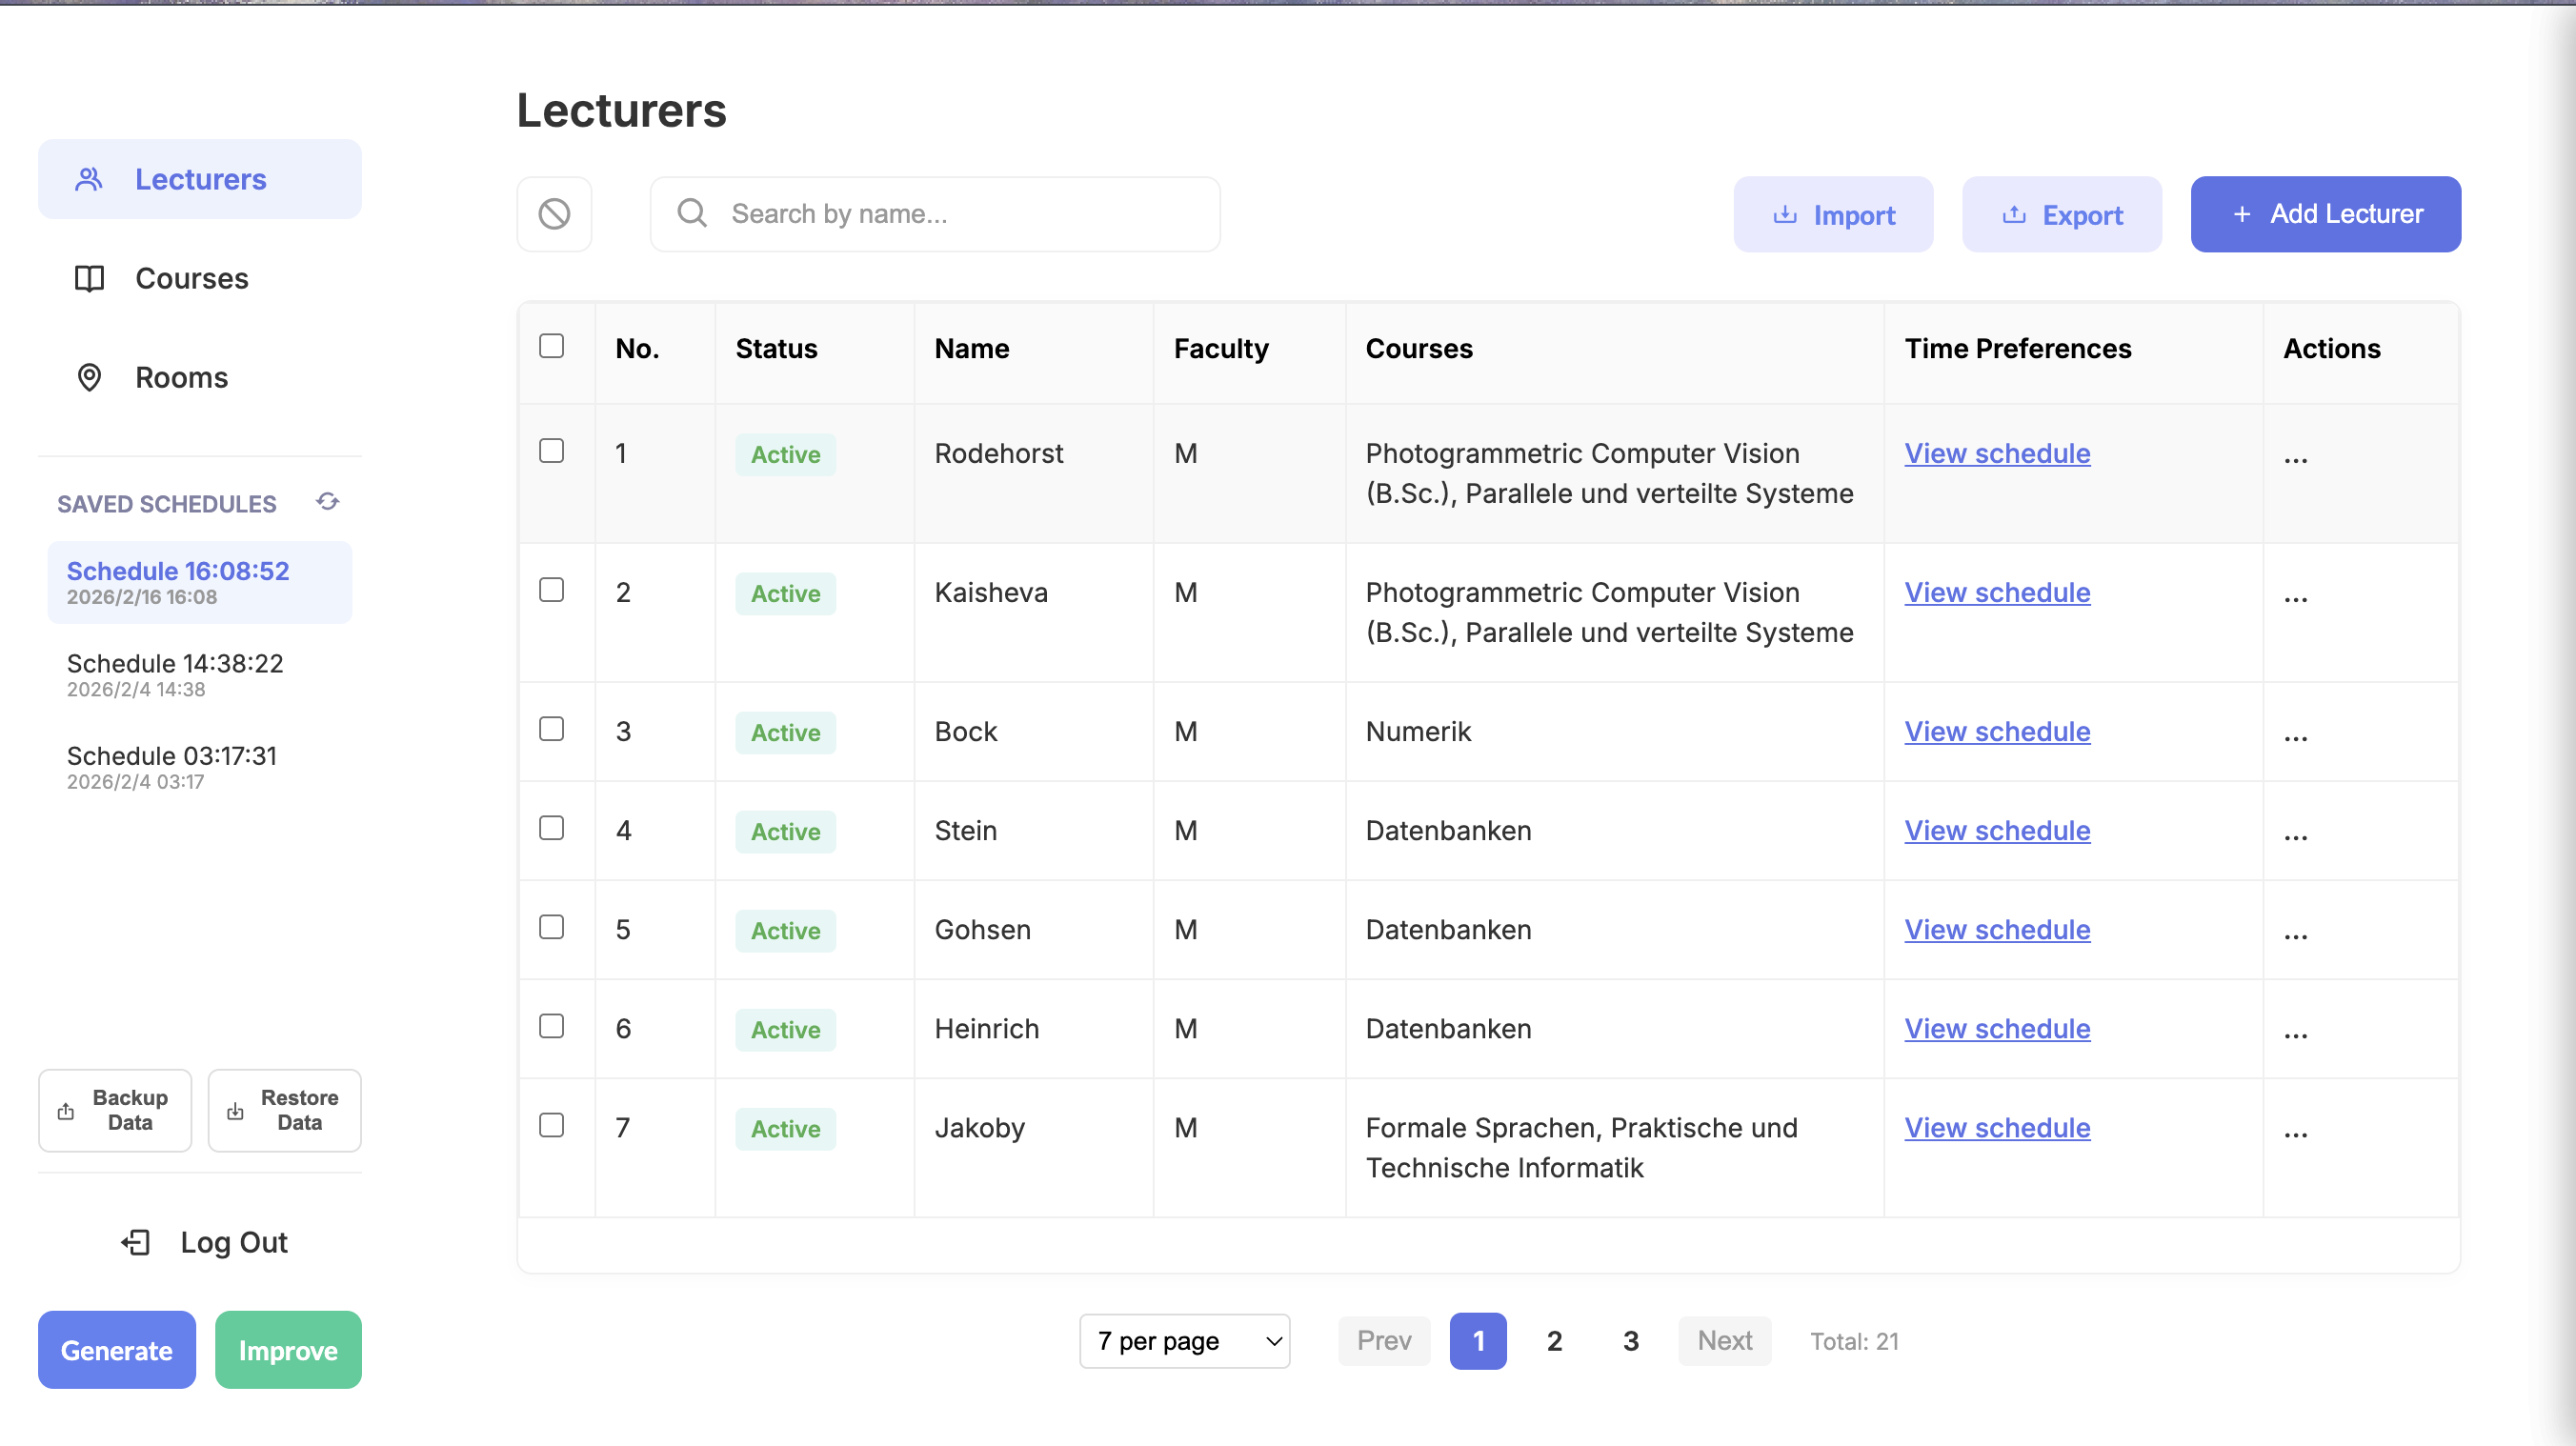
\includegraphics[width=0.9\textwidth]{png/ui_main_dashboard.png}
    \caption{The OpTime main control panel, illustrating the side-panel version control and the responsive data management table.}
    \label{fig:dashboard}
\end{figure}

\subsection{The Multi-Dimensional Availability Matrix}
To address the inherent complexity of faculty time preferences, we developed an \textbf{Interactive Availability Matrix} (see Figure \ref{fig:matrix}). This component acts as the primary interface for translating human availability into mathematical constraints.
\begin{itemize}
    \item \textbf{Grid-Based Selection}: The matrix covers a 7-day week with predefined 90-minute time slots (spanning from 07:30 to 20:30). Each cell is an interactive toggle.
    \item \textbf{Semantic Constraint Categorization}: 
        \begin{itemize}
            \item \textbf{Mint Green (Available)}: Open slots which the solver is encouraged to use.
            \item \textbf{Amber (Preferred - Soft)}: Indicates slots that the "Improve" algorithm should prioritize to maximize lecturer satisfaction.
            \item \textbf{Coral Red (Unavailable)}: Represents hard constraints that the solver is strictly prohibited from occupying.
        \end{itemize}
    \item \textbf{Efficiency Overlays}: The modal includes "Set to Available" and "Reset Schedule" batch actions, significantly reducing the manual labor required to configure a full-week schedule for 20+ lecturers.
\end{itemize}

\begin{figure}[H]
    \centering
    % 注意：这里改成了 png 后缀，并指向 png 文件夹
    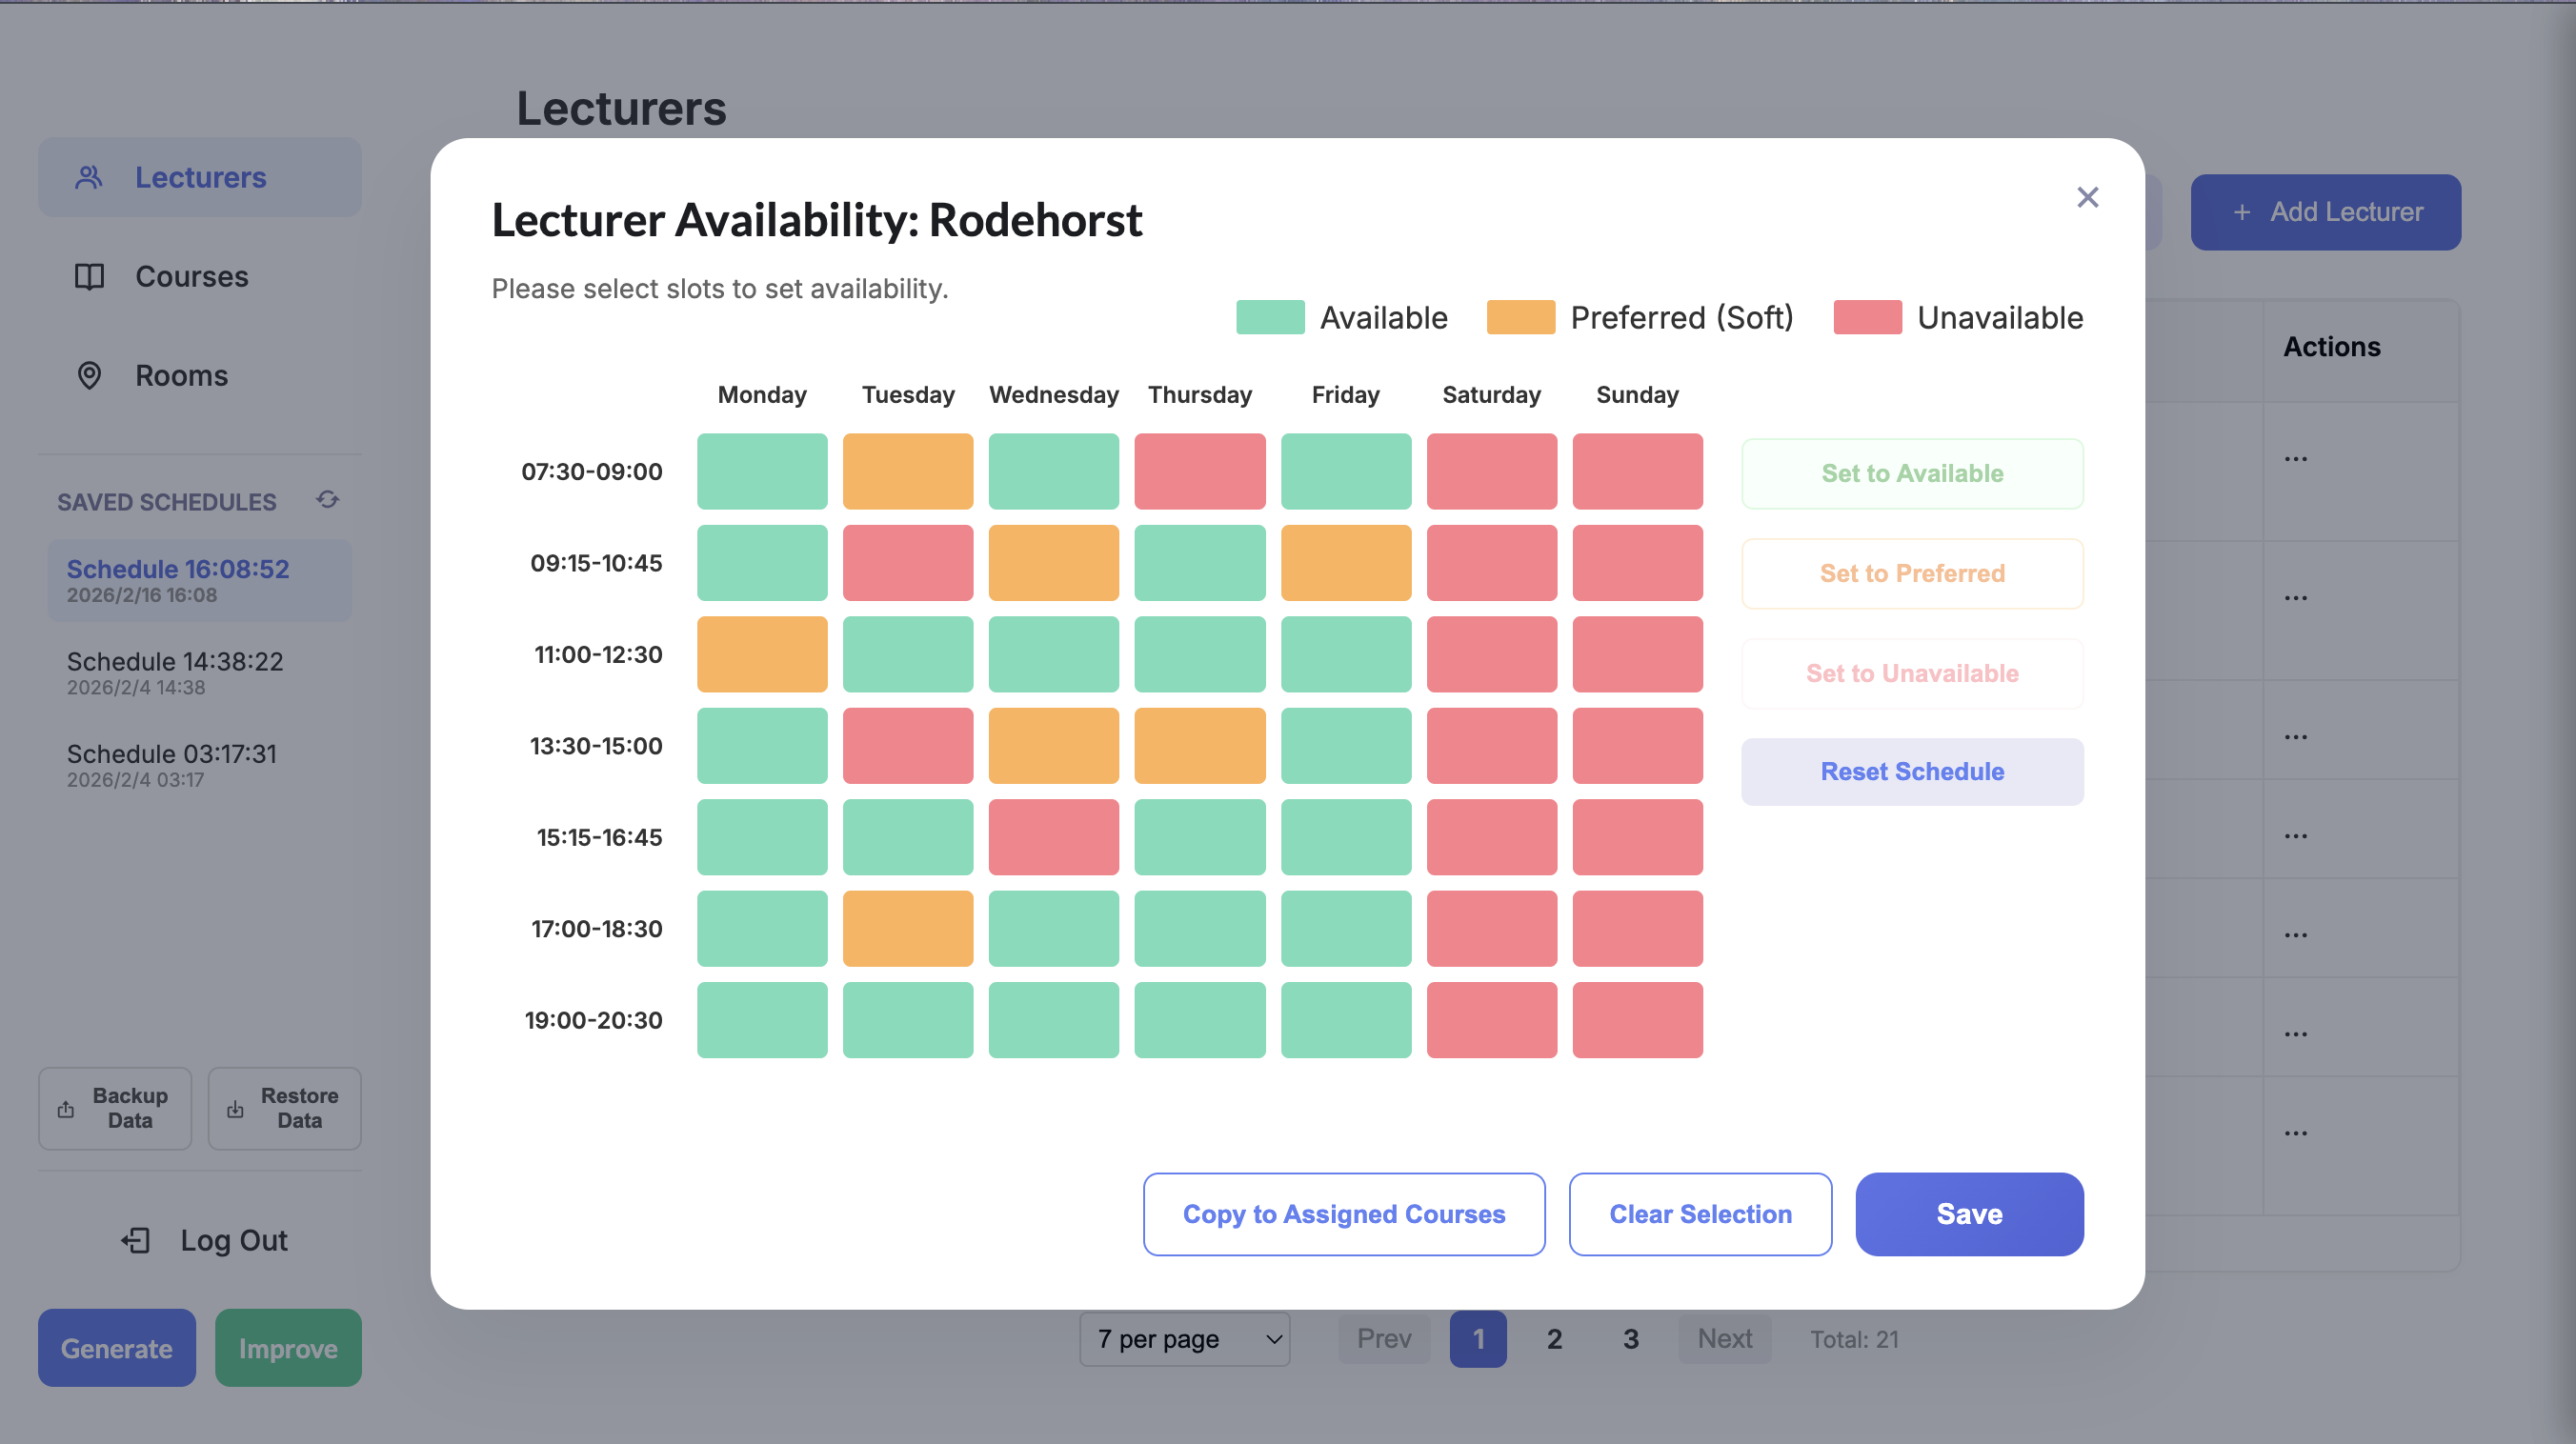
\includegraphics[width=0.8\textwidth]{png/ui_availability_matrix.png}
    \caption{Detailed view of the Lecturer Availability Matrix, showing the three-tier coloring system for hard and soft constraints.}
    \label{fig:matrix}
\end{figure}

\subsection{Contextual Workflow via Dynamic Modals}
Data entry for complex entities is managed through \textbf{Dynamic Overlay Modals} (see Figure \ref{fig:course_modal}), which maintain the user's place in the main list while providing a focused environment for input.
\begin{itemize}
    \item \textbf{Intelligent Field Linking}: The "Add Course" modal allows for multi-lecturer selection and curriculum allocations (e.g., "Mandatory" vs. "Elective"). This ensures that the front-end captures all parameters required by the back-end optimization solver.
    \item \textbf{Real-Time Validation}: The UI provides instant browser-level feedback to ensure data integrity before the information is committed to the database.
\end{itemize}

\begin{figure}[H]
    \centering
    % 注意：这里改成了 png 后缀，并指向 png 文件夹
    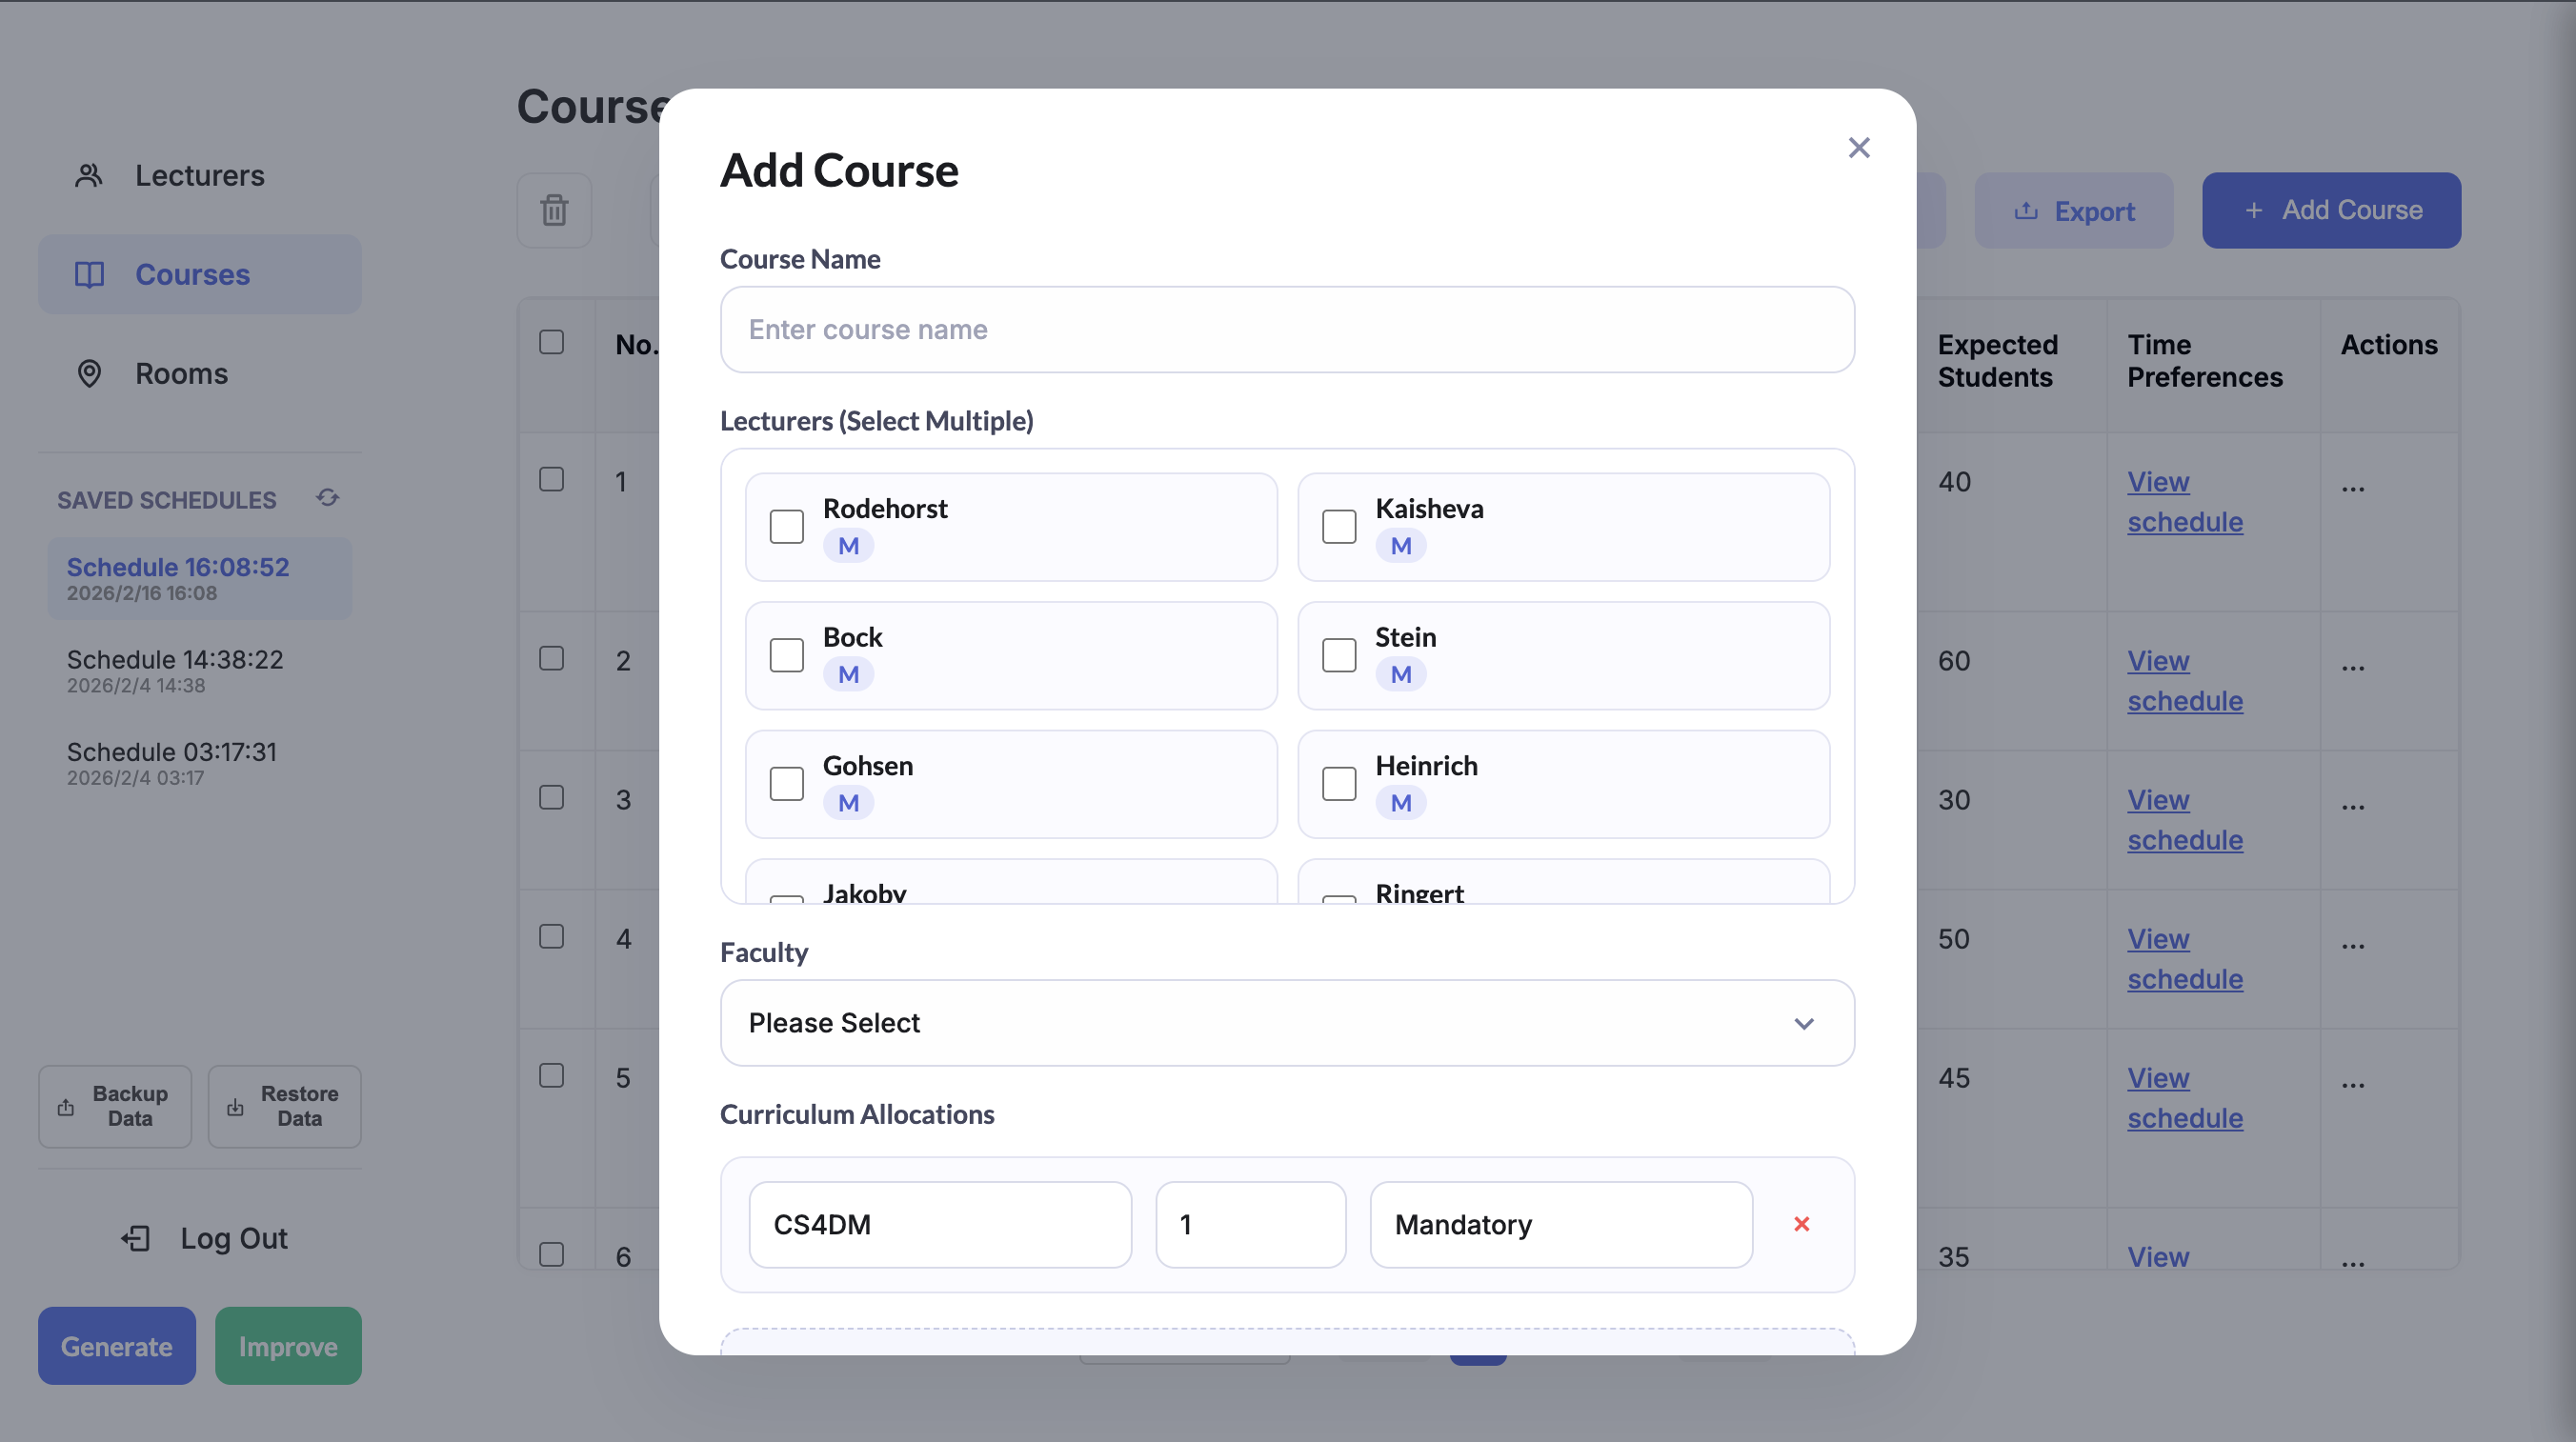
\includegraphics[width=0.8\textwidth]{png/ui_add_course_modal.png}
    \caption{The "Add Course" modal demonstrating multi-select lecturer logic and curriculum allocation fields.}
    \label{fig:course_modal}
\end{figure}

\subsection{Output Visualization: The Generated Timetable}
The final product of the OpTime system is rendered in a \textbf{Dynamic Weekly Planner} format (see Figure \ref{fig:timetable}), transforming raw solver data into a human-readable schedule.
\begin{itemize}
    \item \textbf{Contextual Course Cards}: Each session card is automatically color-coded and displays essential metadata: Course Name, Lecturer, and Room Code.
    \item \textbf{The Diagnostic Gateway}: A high-visibility \textbf{"View Report"} button (Red) provides access to a detailed modal that categorizes any soft conflicts, allowing for transparent "Human-in-the-loop" decision making.
\end{itemize}

\begin{figure}[H]
    \centering
    % 注意：这里改成了 png 后缀，并指向 png 文件夹
    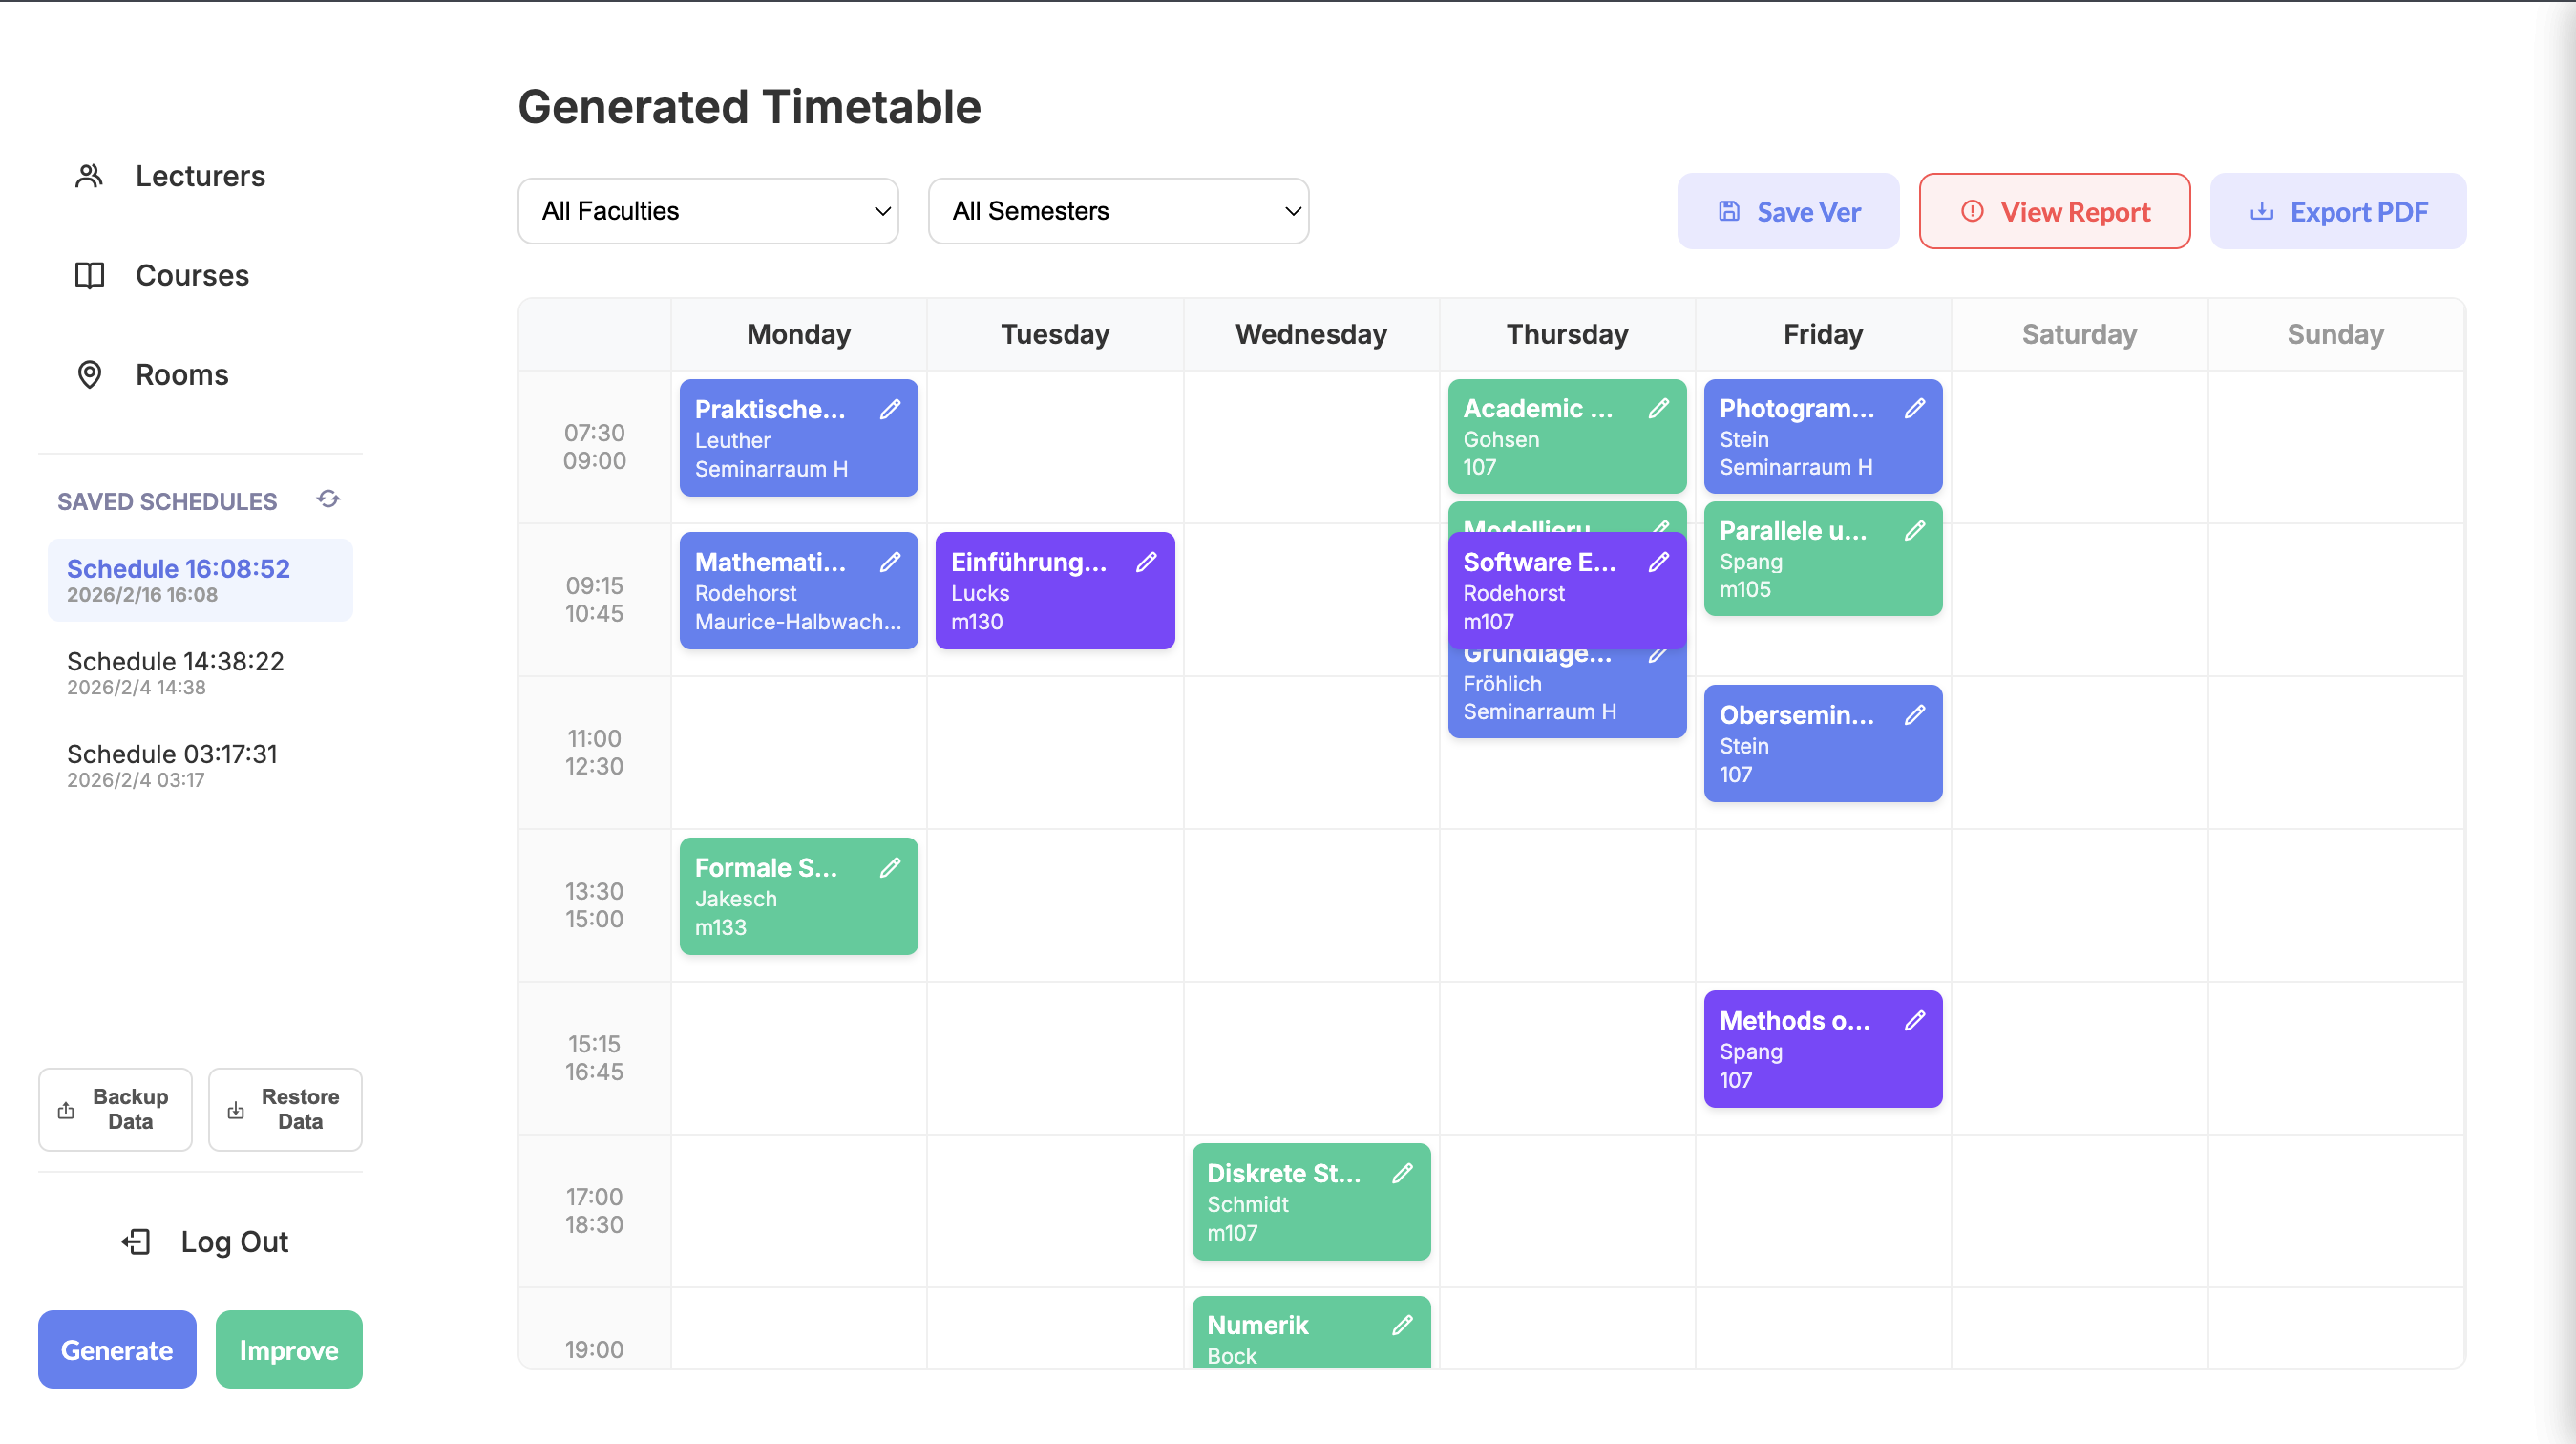
\includegraphics[width=0.9\textwidth]{png/ui_generated_timetable.png}
    \caption{The final generated timetable, showcasing the adaptive 2D grid and the diagnostic reporting triggers.}
    \label{fig:timetable}
\end{figure}

\newpage

\section{Technical Implementation}

\subsection{Front-End Architecture}
The front-end is developed using a component-based approach to ensure scalability. By separating the logic for the \textbf{Data Tables}, \textbf{Schedule Grid}, and \textbf{Notification Modals}, we achieved a highly responsive system.
\begin{itemize}
    \item \textbf{Framework}: JavaScript (ES6+) for dynamic DOM manipulation and state management.
    \item \textbf{Styling}: Custom CSS3 with Flexbox and Grid for the timetable's complex 2D-layout.
\end{itemize}

\subsection{The Dynamic Timetable Engine}
The most technically demanding feature is the \textbf{Interactive Schedule Grid} (as shown in the simulation):
\begin{itemize}
    \item \textbf{State-Driven Rendering}: The grid dynamically maps JSON-formatted schedule data into visual "Course Cards." Each card’s position is calculated based on its time-slot and day index.
    \item \textbf{Conflict Visualization}: We implemented a real-time validation layer. When the system detects a scheduling overlap (e.g., a lecturer assigned to two rooms at once), the card's border color triggers a state change to \textbf{Red}, providing immediate UI feedback.
    \item \textbf{Drag-and-Drop Interaction}: Users can manually override the algorithm by moving cards. The system re-validates the constraints on every "drop" event.
\end{itemize}

\subsection{Asynchronous Operation Handling}
To maintain a smooth user experience during heavy computations:
\begin{itemize}
    \item \textbf{Loading States}: During the "Improve Schedule" phase, an animated overlay provides visual feedback that the back-end optimization algorithm is processing.
    \item \textbf{Promise-based API Calls}: Used \texttt{fetch} to communicate with the server-side solver, allowing the UI to remain interactive while waiting for the optimized timetable result.
\end{itemize}

\newpage

\section{Data Interaction \& Integration}

\subsection{Bridge Between User and Algorithm}
The front-end acts as a sophisticated visual interpreter for the back-end optimization solver. The integration focuses on converting raw mathematical constraints into actionable user information.

\subsection{Intelligent Conflict Reporting}
One of the system's core strengths is the \textbf{Generation Report} modal (as seen in the workflow):
\begin{itemize}
    \item \textbf{Categorized Feedback}: The front-end parses JSON response logs into two distinct categories: 
        \begin{itemize}
            \item \textbf{Critical Issues}: (Red) Logical impossibilities, such as "Lecturer Availability Conflict."
            \item \textbf{Preference Warnings}: (Yellow) Soft constraint violations, such as "Insufficient Room Capacity" or building mismatches.
        \end{itemize}
    \item \textbf{Traceability}: Each error message is linked to specific IDs, allowing users to pinpoint which course or room requires manual adjustment.
\end{itemize}

\subsection{Optimization Workflow \& Persistence}
\begin{itemize}
    \item \textbf{Iterative Improvement}: The \textbf{"Improve"} button triggers a POST request that sends the user's manual adjustments back to the solver. This creates a "Human-in-the-loop" optimization cycle where the AI refines the user's manual layout.
    \item \textbf{Data Export}: Integrated a PDF generation library that captures the high-fidelity CSS grid of the timetable and converts it into a print-ready document via the \textbf{"Export PDF"} trigger.
    \item \textbf{State Persistence}: Implemented "Backup" and "Restore" functionality to ensure that complex scheduling progress is saved to the local storage or database, preventing data loss.
\end{itemize}

\subsection{Final Summary}
Our front-end solution successfully bridges the gap between complex algorithmic outputs and intuitive academic management. By providing real-time visual feedback and structured reporting, we have transformed a high-dimensional optimization problem into a manageable, user-friendly administrative tool.

\end{document}